% Slides for TSD day

\documentclass{beamer} % oral talk
%\documentclass[trans]{beamer}  % paper version
\mode<presentation> {
  %\usetheme{Darmstadt}
  \usetheme{Madrid}
  \usecolortheme{crane}
  %\usetheme{Goettingen}
  %\usecolortheme{wolverine}
  \setbeamercovered{transparent}
  %\useoutertheme{sidebar}
}
\usepackage{graphicx}
\usepackage{xspace}
\usepackage[dvips]{epsfig}
\usepackage{xmpmulti}
\usepackage{color}
\usepackage{colortbl}
\usepackage{setspace}
\usepackage{array}
\usepackage{latexsym}
\usepackage{comment}
\usepackage{amssymb,amsmath,amsthm}
\usepackage{ulem}
\usepackage{extarrows}

\usepackage {bussproofs}
\bottomAlignProof

\usepackage{dednatcol}
\usepackage{alltt}
\usepackage[latin1]{inputenc}
\usepackage{times}
\usepackage[T1]{fontenc}
\usepackage[english]{babel}

\definecolor{Blue}{rgb}{0.1,0.1,0.8}

\newcommand{\keywd}[1]{\textbf{#1}}

\setbeamercovered{dynamic}
\setbeamertemplate{theorems}[numbered]

\newcommand{\hs}{\hspace{1cm}}
\newcommand{\vs}{\vspace{1cm}}
\newcommand{\vsfive}{\vspace{5mm}}
\newcommand{\hsfive}{\hspace{5cm}}

\newcommand{\mboxfill}{\mbox{ }\hfill}

% Variables logiques

\newcommand{\rv}{\bleu {rv}\xspace}
\newcommand{\re}{\bleu {re}\xspace}
\newcommand{\rg}{\bleu {rg}\xspace}
\newcommand{\rd}{\bleu {rd}\xspace}

\newcommand{\pv}[1]{{\bleu {\textsf{I}}(\marron{#1})}}
\newcommand{\pe}[1]{{\bleu {\textsf{W}}(\marron{#1})}}
\newcommand{\pg}[1]{{\bleu {\textsf{S}}(\marron{#1})}}
\newcommand{\pd}[1]{{\bleu {\textsf{D}}(\marron{#1})}}

\newcommand{\vv}[1]{{\bleu {I}(\ensuremath{\vav{#1}})}}
\newcommand{\ve}[1]{{\bleu {W}(\ensuremath{\vav{#1}})}}
\newcommand{\vg}[1]{{\bleu {S}(\ensuremath{\vav{#1}})}}
\newcommand{\vd}[1]{{\bleu {D}(\ensuremath{\vav{#1}})}}

\newcommand{\mystrut}{\hbox to 0pt{\phantom{()}}}
%%%%%%%%%%%%%%%%%


\newtheorem{defn}{Definition}


%\newtheorem{theo}{Theorem}[section] % theorems are numbered by section
\newtheorem{theo}{Theorem} % theorems are numbered by section
\newtheorem{prop}[theo]{Proposition} % propositions are numbered as theorems
\newtheorem{lem}{Lemma} % lemmas are no longer numbered as theorems
\newtheorem{myfact}[theo]{Fact} % lemmas are numbered as theorems
\newtheorem{de}[theo]{Definition} % 

% \newcommand{\egdef}%
%    {\ensuremath{~\:\mathrel{\raisebox{-.7ex}%
%    {$\stackrel{\rm def}{=\mkern-8mu=}$}}\:~}}

\renewcommand{\impl}{\ensuremath{\Rightarrow}}


% \definecolor{marron}{rgb}{0.6, 0.2, 0}
% \definecolor{mygreen}{rgb}{0.0,0.5,0.0}
% \definecolor{brique}{rgb}{0.75, 0.05, 0}
% \definecolor{violet}{rgb}{.75, 0, .75}

% \definecolor{lightblue}{rgb}{0.75,0.85,1}
% \definecolor{lightred}{rgb}{1,0.8,0.8}
% \definecolor{lightgreen}{rgb}{0.6,1,0.6}
% \definecolor{semilightgreen}{rgb}{0.5,1,0.5}
% \definecolor{lightyellow}{rgb}{1.0,1.0,0.5}
% \definecolor{lightorange}{rgb}{1.0, 0.87, 0.01}

% \newcommand{\marron}[1]{\textcolor{marron}{#1}}
% \newcommand{\brun}[1]{\textcolor{brown}{#1}}
% \newcommand{\cvert}[1]{\textcolor{mygreen}{#1}}
% \newcommand{\bleu}[1]{\textcolor{blue}{#1}}
% \newcommand{\rouge}[1]{\textcolor{red}{#1}}
% \newcommand{\brique}[1]{\textcolor{brique}{#1}}
% \newcommand{\violet}[1]{\textcolor{violet}{#1}}

\newcommand{\cdat}{\violet}
\newcommand{\cloc}{\cvert}

% ----------------------------------------------------------------------
\newcommand{\loc}{\cloc{\textit{loc}}}
\newcommand{\lx}{\cloc{\textit{x}}}
\newcommand{\ly}{\cloc{\textit{y}}}

\newcommand{\edge}[2]{\ensuremath{\cloc{#1\!\mathbin{\rightarrow}\! #2}}}
\newcommand{\cdb}{\ensuremath{\mathcal{\cdat C}}}
\newcommand{\incdb}[1]{\ensuremath{#1\in\cdb}}
\newcommand{\nincdb}[1]{\ensuremath{#1\not\in\cdb}}
\newcommand{\cdbp}{\ensuremath{\cdat{\mathcal{C}'}}}
\newcommand{\incdbp}[1]{\ensuremath{#1\in\cdbp}}
\newcommand{\nincdbp}[1]{\ensuremath{#1\not\in\cdbp}}
\newcommand{\atloc}[1]{\cdat{\ensuremath{\left|\cloc{#1}\right|}}}
\newcommand{\inset}[2]{\ensuremath{#1\in#2}}
\newcommand{\inloc}[2]{\ensuremath{#1\in\atloc{#2}}}
\newcommand{\ninloc}[2]{\ensuremath{#1\not\in\atloc{#2}}}
\newcommand{\visloc}[2]{\ensuremath{#1\in\cdat{\overline{\atloc{#2}}}}}
\newcommand{\nvisloc}[2]{\ensuremath{#1\not\in\cdat{\overline{\atloc{#2}}}}}
\newcommand{\inedge}[3]{\inloc{#1}{\edge{#2}{#3}}}
\newcommand{\ninedge}[3]{\ninloc{#1}{\edge{#2}{#3}}}
\newcommand{\cnf}{\textit{\cdat{cnf}}}
\newcommand{\pre}{\cdat{\textit{pre}}}
\newcommand{\post}{\cdat{\textit{post}}}
\newcommand{\extconfpar}[2]{\cdat{\ensuremath{\langle #1, #2\rangle}}}
\newcommand{\extconf}{\extconfpar{\cnf}{\cdb}}
\newcommand{\extconfpre}{\extconfpar{\pre}{\cdb}}
\newcommand{\extconfpost}{\extconfpar{\post}{\cdbp}}
%\newcommand{\entails}{~\rhd~}
\newcommand{\entailstrans}{\:\xrightarrow{\:trans\:}\:} % general
\newcommand{\entailsp}{\:\xrightarrow{\:sr\:}\:} % pure synchronous round
\newcommand{\entailso}{\:\xrightarrow{\:or\:}\:} % oracle round
\newcommand{\entails}{\:\xrightarrow{\:sor\:}\:} % synchronous + oracle round
\newcommand{\roas}{\textsc{roas}}
\newcommand{\roasat}[2]{\ensuremath{\roas\,@\,\edge{#1}{#2}}}
\newcommand{\roasto}[1]{\ensuremath{\roas\,@\,\cloc{\overline{#1}}}}
\newcommand{\goodat}[2]{\ensuremath{good\,@\,\edge{#1}{#2}}}
\newcommand{\goodto}[1]{\ensuremath{good\,@\,\cloc{\overline{#1}}}}
\newcommand{\correctonSTat}[1]{\ensuremath{\mbox{correct-onST}\,@\,\cloc{#1}}}
\newcommand{\wcorrectonSTat}[1]{\ensuremath{\mbox{weak-correct-onST}\,@\,\cloc{#1}}}
\newcommand{\completeonSTat}[1]{\ensuremath{\mbox{complete-onST}\,@\,\cloc{#1}}}
\newcommand{\readyat}[1]{\ensuremath{\mbox{ready}\,@\,\cloc{#1}}}
\newcommand{\correctSTat}[1]{\ensuremath{\mbox{correct-ST}\,@\,\cloc{#1}}}
\newcommand{\completeSTat}[1]{\ensuremath{\mbox{complete-ST}\,@\,\cloc{#1}}}
\newcommand{\invarat}[1]{\ensuremath{\mbox{invar}\,@\,\cloc{#1}}}


\newcommand{\hcinv}{\texttt{hc\_inversion}\xspace}

% Front page

\title{Certification of C programs with Compcert for SimSoC}

%\subtitle{No subtitle}
\author[X. Shi] % (optional, nur bei vielen Autoren)
{Fr\'{e}d\'{e}ric Blanqui\\Vania Joloboff\\Jean-Fran\c{c}ois Monin\\\underline{Xiaomu Shi}\\Fr\'{e}d\'{e}ric Tuong\\}

\institute[LIAMA \& Univ Grenoble]

\date[April 26th, 2013]

\begin{document}

\frame{\titlepage

\vfill

}

\section<presentation>*{Outline}

\begin{frame}
  \frametitle{Outline}
  \setcounter{tocdepth}{2}
  \tableofcontents%[part=1,pausesections]
\end{frame}


%\AtBeginSubsection[] {
\AtBeginSection[] {
  \begin{frame}<beamer>
    \frametitle{Outline}
    \setcounter{tocdepth}{2}
    \tableofcontents[current,subsection]
  \end{frame}
}


%%%%%%%%%%%%%%%%%%%%%%%%%%%%%%%%%%%%%%%%%%%%%%%%%%%
%%%%%%%%%%%%%%%%%%%%%%%%%%%%%%%%%%%%%%%%%%%%%%%%%%%
\section{Introduction}

%%%%%%%%%%%%%%%%%%%%%%%%%%%%%%%%%%%%%%%%%%%%%%%%%%%

\subsection{Certifying C programs}

\begin{frame}
\frametitle{Popular approaches for certifying a C program}
\begin{block}
{Tools based on axiomatic semantics (Hoare logic)}
Frama-C: a platform for C
program static analysis and automatic deductive verification
\end{block}
\bigskip
\pause
\textcolor{blue}{%
Difficult to express complex specifications and expected
properties at the right abstraction level
}
\end{frame}

\begin{frame}
\frametitle{Using CompCert C for C program certification}
%have not been tried until our approach
\begin{block}
{Operational semantics based approach}
CompCert C: Coq-certified C compiler (developed at INRIA),\\
            large subset of C language
\end{block}
\bigskip
\pause
\textcolor{blue}{%
Accurate and rich enough to express our large specification,\\
containing a formal model of ARM V6 for SimSoC
}
\end{frame}

\subsection{Certification target, SimSoC}

\begin{frame}
\frametitle{The C++ open-source, SimSoC}
\begin{block}{Goal}
SimSoc: Simulator of System-On-Chip
\end{block}
\begin{block}{Features}
\begin{itemize}
\item Simulates various architectures: ARM PPC MIPS SH4
\item 60,000 lines of C++ and SystemC
\item Over 10 millions instructions per second
\item Loosely-timed
\item Includes optimizations, like dynamic translation
\item Can run Linux both on ARM and PowerPC architectures
\end{itemize}
\end{block}
\bigskip
Complementary to the simulator presented in the first talk yesterday
\end{frame}

\begin{frame}
\frametitle{The ARM simulation module}

\begin{block}{ARM programmer's model}
\begin{itemize}
\item ARM processor
\item 147 ARM instructions
\item 5 kinds of addressing mode
\item System Control Coprocessor (CP15)
\item Memory Management Unit (MMU)
\end{itemize}
\end{block}
\bigskip
ARMv5 is manually implemented
\end{frame}

\begin{frame}
\frametitle{A light version in C, Simlight}
\begin{block}{ARM programmer's model}
\begin{itemize}
\item ARM processor
\item 147 ARM instructions
\item 5 kinds of addressing mode
\item \sout{System Control Coprocessor (CP15)}
\item \sout{Memory Management Unit (MMU)} $\rightarrow$ Simplified memory model 
\end{itemize}
\end{block}
\bigskip
ARMv6 instructions are automatically generated
\end{frame}


%%%%%%%%%%%%%%%%%%%%%%%%%%%%%%%%%%%%%%%%%%%
\section{SimSoC-Cert}

%%%%%%%%%%%%%%%%%%%%%%%%%%%%%%%%%%%%%%%%%%%

\subsection{Overall architecture of SimSoC-Cert}
\begin{frame}
\frametitle{Overall architecture of SimSoC-Cert}
\hfil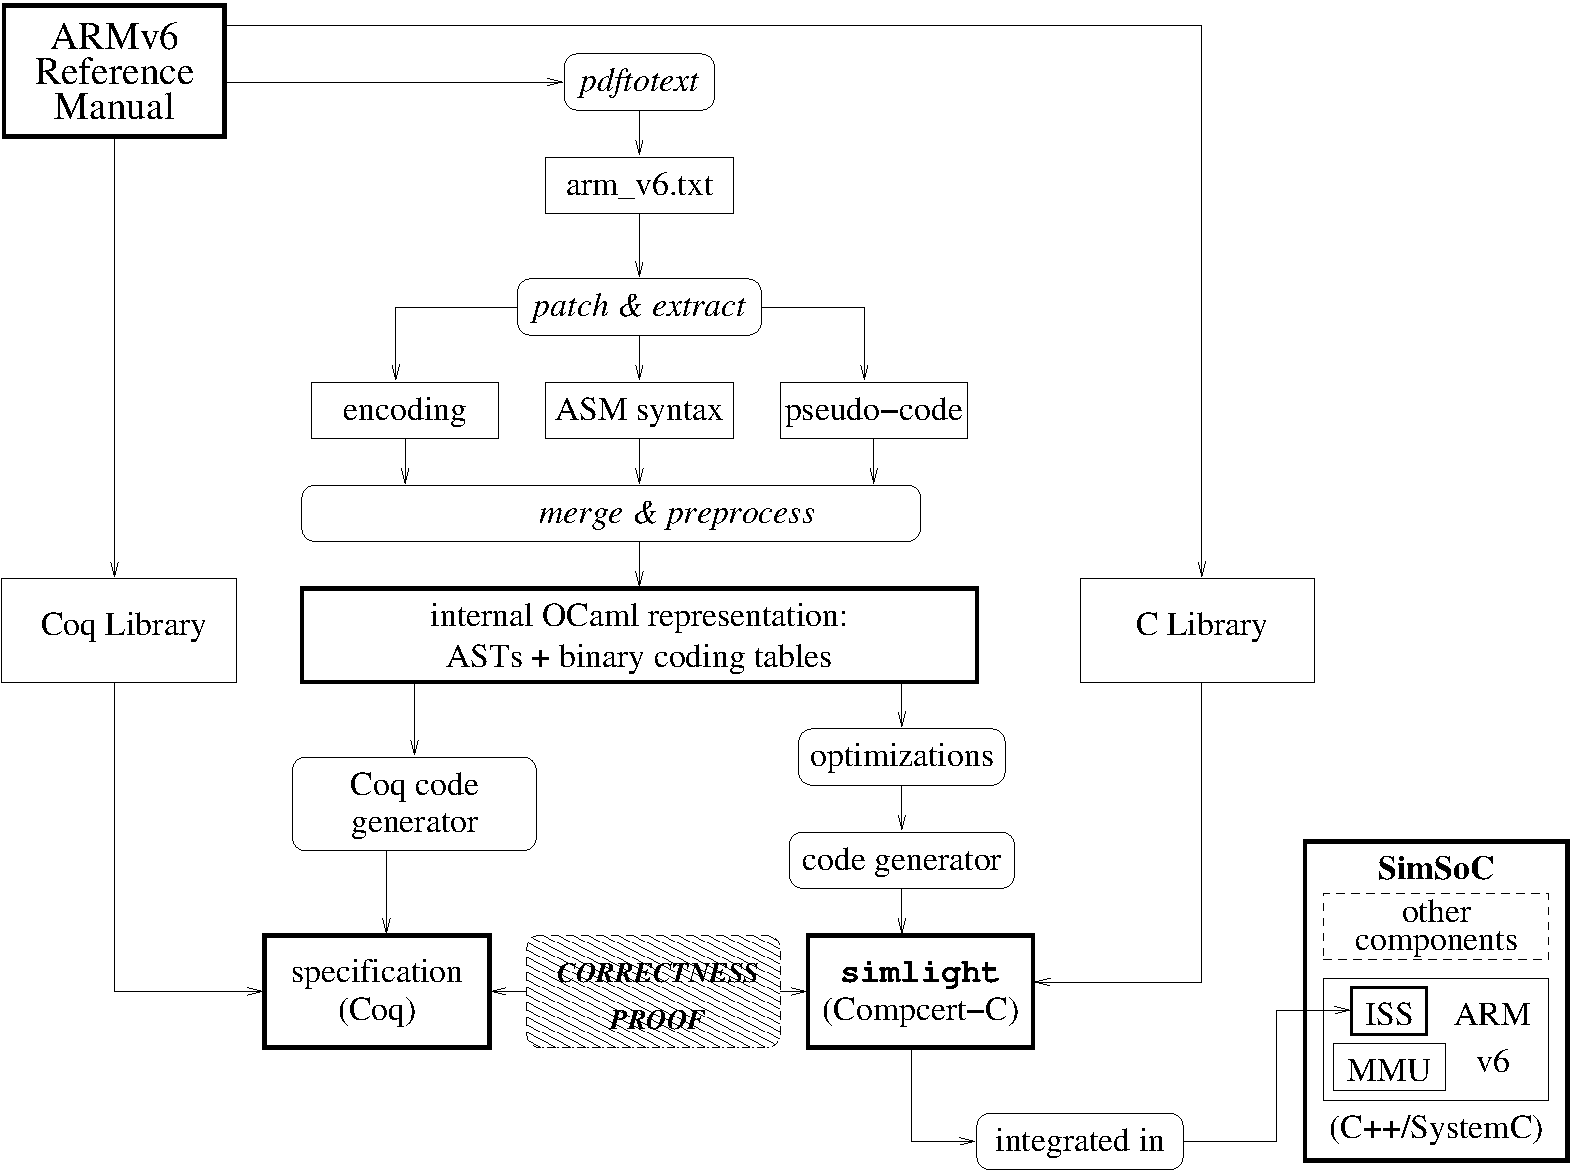
\includegraphics[width=.8\linewidth]{fullarchi.pdf}
\end{frame}

\subsection{ARM model}

\begin{frame}[fragile]
\frametitle{ARMv6 ref manual: instruction ADC in pseudo-code}
%code of ADC
\begin{alltt}
A4.1.2 ADC
  \bleu{if} ConditionPassed(cond) \bleu{then}
    \textbf{Rd = Rn + shifter_operand + C Flag;}
    \bleu{if} S == 1 and d == 15 \bleu{then}
      \bleu{if} CurrentModeHasSPSR() \bleu{then}
          CPSR = SPSR;
      \bleu{else} UNPREDICTABLE
    \bleu{else} \bleu{if} S == 1 \bleu{then}
      N Flag = Rd[31];
      Z Flag = \bleu{if} Rd == 0 \bleu{then} 1 \bleu{else} 0;
      C Flag = CarryFrom(Rn + shifter_operand
                            + C Flag);
      V Flag = OverflowFrom(Rn + shifter_operand
                               + C Flag);

\end{alltt}
\end{frame}

\begin{frame}[fragile]
\frametitle{Coq specification of ARM instruction ADC}
\small
\begin{alltt}
(* A4.1.2 ADC *)
Definition ADC_step
    (S : bool) (cond : opcode) (d : regnum) (n : regnum)
    (shifter_operand : word) : semfun _ := 
  \brique{<s0>} \bleu{if}_\bleu{then} (ConditionPassed s0 cond)
    ([ \brique{<st>} set_reg d (add (add (reg_content s0 n)
                                shifter_operand)
                                ((cpsr st)[Cbit]))
    ; \bleu{If} (andb (zeq S 1) (zeq d 15))
       \bleu{then}
           (\brique{<st>} if_CurrentModeHasSPSR (fun em =>
              (\brique{<st>} set_cpsr (spsr st em))))
\tiny
            \bleu{else}         (\bleu{if_then} (zeq S 1)
                ([ \brique{<st>} set_cpsr_bit Nbit ((reg_content st d)[n31])
                ; \brique{<st>} set_cpsr_bit Zbit (\bleu{if} zeq (reg_content st d) 0 \bleu{then} repr 1 
                                          \bleu{else} repr 0)
                ; \brique{<st>} set_cpsr_bit Cbit
                          (CarryFrom_add3 (reg_content s0 n) shifter_operand
                                          ((cpsr st)[Cbit]))
                ; \brique{<st>} set_cpsr_bit Vbit (OverflowFrom_add3 (reg_content s0 n)
                                     shifter_operand ((cpsr st)[Cbit])) ])) ]).
\end{alltt}
\end{frame}
\begin{frame}[fragile]
\frametitle{Coq representation of CompcertC AST}
\newcommand{\mycirc}{\begin{math}\circ\end{math}}
\newcommand{\tbs}{\textbackslash}
\newcommand{\mabullet}{\begin{math}\bullet\end{math}}
\small
\begin{alltt}
Definition ADC\_Coq\_simlight := (ADC, Internal 
    \{| fn_return := void; fn_params := \tiny
         [proc -: `*` typ_SLv6_Processor; 
          S -: uint8; cond -: int32; d -: uint8; n -: uint8; 
          shifter_operand -: uint32];
         fn_vars := [ old_Rn -: uint32];\small
      fn_body :=
($ old_Rn`:\mycirc) `= (call (\tbs{}reg`:\mycirc) E[\tbs{}proc`:\mycirc; \tbs{}n`:\mycirc] \mycirc)`:\mycirc;;
\bleu{`if}\,(\mabullet\,(\tbs{}ConditionPassed`:\mycirc)\,E[&((`*(\tbs{}proc`:\mycirc)`:\mycirc)|cpsr`:\mycirc)`:\mycirc;\,\tbs{}cond`:\mycirc] \mycirc)
 \bleu{then} (\mabullet\,(\tbs{}set_reg_or_pc`:\mycirc) E[\tbs{}proc`:\mycirc; \tbs{}d`:\mycirc; ((\tbs{}old_Rn`:\mycirc)+\mabullet)+\mabullet:\mycirc]\,\mycirc);;
 \bleu{`if} ((($ S`:\mycirc)==(#1`:\mycirc)`:\mycirc)&(($ d`:\mycirc)==(#15`:\mycirc)`:\mycirc)`:\mycirc)\tiny
     \bleu{then} \bleu{`if} (call (\tbs{}CurrentModeHasSPSR`:\mycirc) E[\tbs{}proc`:\mycirc] \mycirc)
      \bleu{then} (call (\tbs{}copy_StatusRegister`:\mycirc) E[&(\mabullet|cpsr`:\mycirc)`:\mycirc; \mabullet] \mycirc)
      \bleu{else} (call ($ unpredictable`:\mycirc) E[] \mycirc)
     \bleu{else} \bleu{`if} (($ S`:\mycirc)==(#1`:\mycirc)`:\mycirc)
      \bleu{then} ((($ proc`:\mycirc)|cpsr`:\mycirc)|N_flag`:\mycirc) `= 
       (\mabullet\,(\tbs{}get_bit`:\mycirc) E[(\mabullet\,(\tbs{}reg`:\mycirc) E[\tbs{}proc`:\mycirc; \tbs{}d`:\mycirc] \mycirc); #31`:\mycirc] \mycirc)`:\mycirc;;
           ((($ proc`:\mycirc)|cpsr`:\mycirc)|Z_flag`:\mycirc) `= 
       (((\mabullet (\tbs{}reg`:\mycirc) \mabullet \mycirc)==(#0`:\mycirc)`:\mycirc)?(#1`:\mycirc)`:(#0`:\mycirc)`:\mycirc)`:\mycirc;;
           ((($ proc`:\mycirc)|cpsr`:\mycirc)|C_flag`:\mycirc) `= 
       (\mabullet (\tbs{}CarryFrom_add3`:\mycirc) E[\mabullet; \mabullet; (\mabullet (\mabullet|C_flag`:\mycirc) \mycirc)] \mycirc)`:\mycirc;;
           ((($ proc`:\mycirc)|cpsr`:\mycirc)|V_flag`:\mycirc) `= 
       (\mabullet (\tbs{}OverflowFrom_add3`:\mycirc) E[(\mabullet (\tbs{}old_Rn`:\mycirc) \mycirc); \mabullet; \mabullet] \mycirc)`:\mycirc
   \bleu{else} skip
 \bleu{else} skip |\}).
\end{alltt}
\end{frame}
%$

%%%%%%%%%%%%%%%%%%%%%%%%%%%%%%%%%%%%%%%%%%%
\section{Correctness proof of ARMv6 instruction}

%%%%%%%%%%%%%%%%%%%%%%%%%%%%%%%%%%%%%%%%%%%


\subsection{Differences between two representations}
\begin{frame}
\frametitle{Differences between two representations}
\begin{block}{Different data types}
More complex types in Simlight, for example:\\
Coq model: CPSR = 32 bits word\\
Simlight: CPSR = data structure, 1 byte-field for every significant bit
\end{block}
\begin{block}{Different semantics}
Coq specification: semantics = function\\
Compcert-C: big-step operational semantics = relation
\end{block}
\begin{block}{Semantics operates on different memory models}
Coq model: on a direct representation of processor state\\
Compcert-C: on a C memory state where processor state is stored
\end{block}
\end{frame}

\begin{frame}[fragile]
\frametitle{Differences between two representations}
\begin{block}{CPSR = SPSR}
\begin{itemize}
\item Coq specification:
\begin{alltt}
set_cpsr (spsr st em)
\end{alltt}
\item CompCert C AST:
\begin{alltt}\small
(Ecall (Evalof (Evar \bleu{copy_StatusRegister} T14) T14)
   (Econs
      (Eaddrof
         (Efield (Ederef (Evalof (Evar proc T3) T3) T6) 
                 \bleu{cpsr} T7) T8)
            (Econs
               (Ecall (Evalof (Evar \bleu{spsr} T15) T15)
                  (Econs (Evalof (Evar proc T3) T3) 
                   Enil) T8) Enil)) T12)
\end{alltt}
\end{itemize}
\end{block}
\end{frame}

\subsection{Projection of ARMv6 processor state}
\begin{frame}
\frametitle{Projection}
\frametitle{Projection of ARMv6 processor state ~~(excerpt)}
\hfil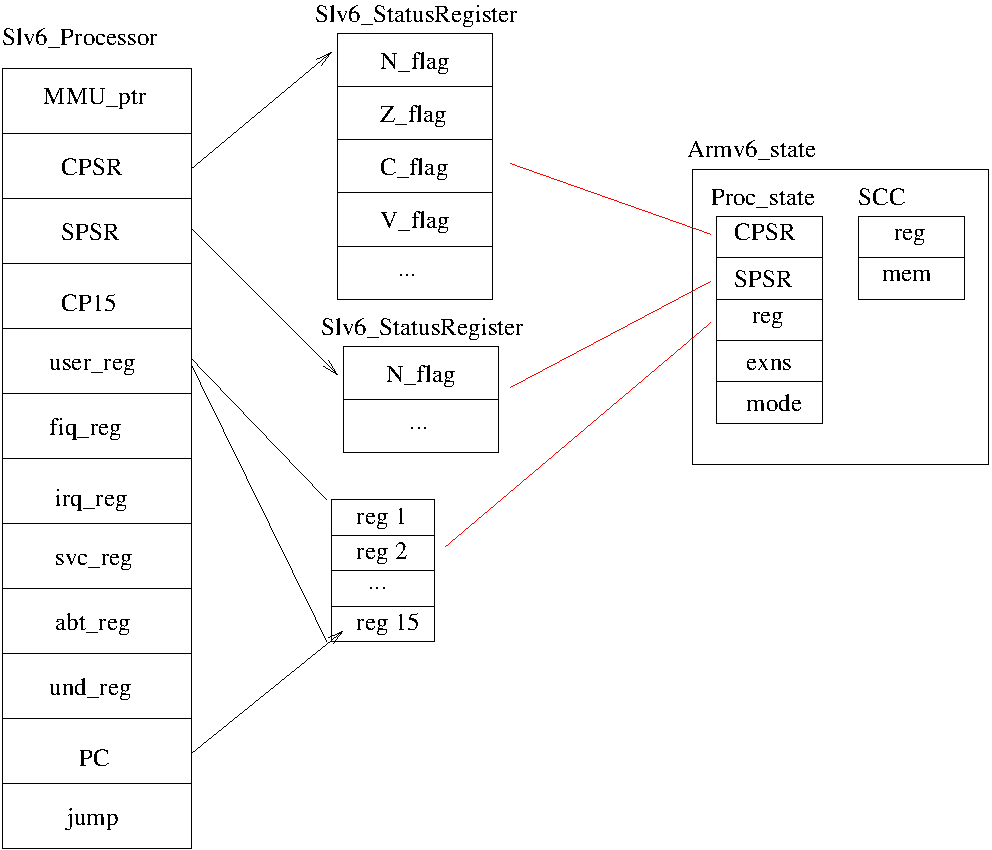
\includegraphics[width=.8\linewidth]{projection.pdf}
\end{frame}

\subsection{Main theorem}
\begin{frame}
\frametitle{Main theorem}
\begin{theorem}
\begin{itemize}
\item $G,empty\_env\vdash \texttt{alloc\_variables},\brique{M0}\overset{vars}{\Rightarrow}\brique{M1},E$
\item $G,E \vdash \texttt{bind\_parameters},\brique{M1} \overset{vargs}{\Rightarrow}\cvert{M}$
\item $\mathit{proc\_state\_related} \: \cvert{M} \: (\texttt{Ok}\: st)$
\item similarly for the arguments of \texttt{ADC}
\item 
  $G,E\vdash \texttt{ADC\_Coq\_simlight},\cvert{M}\overset{t}{\Rightarrow}out,\cvert{M'}$
\end{itemize}
then $\mathit{proc\_state\_related}\: \cvert{M'} \:(\texttt{ADC\_Coq}\: (\mathit{arguments},\:st))$.
\end{theorem}
\end{frame}

\subsection{CompCert C semantics}
\begin{frame}
\frametitle{CompCert C semantics}
\begin{block}{eval\_assign}
\begin{equation}
\frac
{\begin{array}{c}
G,E\vdash l~M\xLongrightarrow{t1}l',M1\qquad
G,E\vdash r~M1\xLongrightarrow{t2}r',M2\\
G,E\vdash l'~M2\Rightarrow (b, ofs)\qquad
G,E\vdash r'~M2\Rightarrow v\\
cast(v,typeof(l),typeof(r))=~\lfloor v'\rfloor\\
store (G,~typeof(l),~M2,~(b,ofs),~v)=~\lfloor M3\rfloor\\
\end{array}
}
{G,E\vdash (l=r)~M\xLongrightarrow{t1**t2**t3}v',M3}
\end{equation}
\end{block}
\begin{block}{eval\_funcall}
\begin{equation}
\frac
{\begin{array}{c}
G,E\vdash rf~M~\xLongrightarrow{t1}~rf',M1\qquad
G,E\vdash rarg^*~M1~\xLongrightarrow{t2}~rarg'^*,M2\\
G,E\vdash M2~rf' \Rightarrow vf\qquad
\texttt{find\_funct}~(G,vf)~=~\lfloor fd\rfloor\\
\vdash M2~fd~varg^* \xLongrightarrow{t3}vres,M3
\end{array}
}
{G,E\vdash M~\langle\textrm{\texttt{Call}}\rangle\xLongrightarrow{t1**t2**t3}vres,M3}
\end{equation}
\end{block}
\end{frame}

\subsection{Technical issue during the proofs}
\begin{frame}
\frametitle{Key technical issue in the proofs}

Correctness proofs based on an operational semantics $\Rightarrow$ \\
reasoning on hypotheses relating objects 
according to this semantics

\medskip

Technically: semantics = inductive type $~\Rightarrow~$ inversion

\medskip

\begin{itemize}
\item
  CompCert C operational semantics : many large rules
\item
  For Simlight : inversions \brique{all over the place!}
\item 
  Coq \texttt{inversion} : \brique{efficiency} and \brique{controllability} issues
\end{itemize}

\medskip

Solution: build our own tactic ~ \bleu{\hcinv} ~ [ITP'13]

\end{frame}

%%%%%%%%%%%%%%%%%%%%%%%%%%%%%%%%%%%%%%%%%%
\section{Conclusion}

%%%%%%%%%%%%%%%%%%%%%%%%%%%%%%%%%%%%%%%%%%%

\subsection{Size of development}
\begin{frame}
\frametitle{Size of development}
\small
\begin{table}[t]
  \centering
  \begin{tabular}{|l|r@{~}|}
    \hline
    Original ARM ref man (txt)           & 49655 \\
    ARM Parsing to an OCaml AST         & \bleu{1068} \\
    Generator (Simgen) for ARM         &   \bleu{10675} \\ 
    General C libraries on ARM         & \bleu{1852} \\ 
    General Coq libraries on ARM         & \bleu{1569} \\ 
    Generated C code for Simlight ARM operations   & \cvert{6681} \\
    Generated Coq code for ARM operations   & \cvert{2068} \\
    Generated Coq code for ARM decoding  & \cvert{592} \\
    Projection   & \bleu{857} \\
    Definition of \hcinv       & \bleu{551} \\
    Definition of other self-defined tactics      & \bleu{185}\\ 
    Proof script on ADC (2011)    & \brique{3171} \\
    Proof scripts on ADC (2012)    & \brique{1204} \\     
%% Xiaomu: please complete
    Proof script on auxiliary functions   & \brique{856} \\
    Proof script on BL (2012)   & \brique{437} \\
    Proof script on MRS (2012)   & \brique{322} \\
    ...\\
    \hline 
  \end{tabular}
  \smallskip
  \caption{Sizes (in loc)}
\end{table}
\end{frame}


\subsection{Future work}
\begin{frame}
\frametitle{Future work}
\begin{itemize}
\item Extend the work to full sets of instructions
\item Proofs for decoder
\item Proofs for simulation loop
\end{itemize}
\end{frame}


\begin{frame}
\begin{center}
{\huge THANKS}
\end{center}

\end{frame}


\end{document}
